% Source for the figure of sidewaysSum() (sec. 18.2): the sums of the
% fields of 2, 4 and 8 bits of a word of 16 bits, formed in place, and the
% sum of its two bytes by the product by 0x0101. Build: make figures (in
% ../build).
\documentclass[border=4pt]{standalone}
\usepackage[T1]{fontenc}
\usepackage{newpxtext,newpxmath}
\usepackage[varqu,varl,scaled=0.95]{zi4}
\usepackage{tikz}
% tikz-ads.tex: the TikZ styles shared by the figures of the memory of the
% manual, \input by each standalone figure: a cell of a vector (cell), the
% cell that an operation touches (touched), a free cell (free), a node of a
% linked structure (node), the labels of indices (index) and of variables
% (var), a pointer (ptr), and \cells and \indices to draw a row of cells.
\usetikzlibrary{arrows.meta,positioning,calc,fit,shapes.multipart}
\definecolor{adsTouched}{RGB}{214,196,236}
\definecolor{adsFree}{RGB}{236,236,236}
\tikzset{
  ads/.style={>={Stealth[length=2mm]},font=\small,
              every node/.append style={inner sep=0pt}},
  cell/.style={draw,minimum width=7mm,minimum height=7mm,
               font=\small\ttfamily,outer sep=0pt},
  touched/.style={cell,fill=adsTouched},
  free/.style={cell,fill=adsFree,text=black!45},
  node/.style={draw,rounded corners=1pt,minimum width=8mm,
               minimum height=6mm,font=\small\ttfamily},
  index/.style={font=\scriptsize\ttfamily,text=black!60},
  var/.style={font=\small\itshape},
  ptr/.style={->,thick}
}
% \cells{name}{x,y}{list}: a row of cells, the first at (x,y), named
% name-0, name-1, ...; each item is text/style, the style one of cell,
% touched and free (e.g., {a/cell,e/touched,/free})
\newcommand{\cells}[3]{%
  \foreach \v/\s [count=\i from 0] in {#3}
    \node[\s] (#1-\i) at ($(#2)+(\i*7mm,0)$) {\v};}
% \indices{name}{n}: the indices 0 .. n-1 under the cells of name
\newcommand{\indices}[2]{%
  \foreach \i in {0,...,\numexpr#2-1\relax}
    \node[index,below=1.2mm of #1-\i] {\i};}

\begin{document}
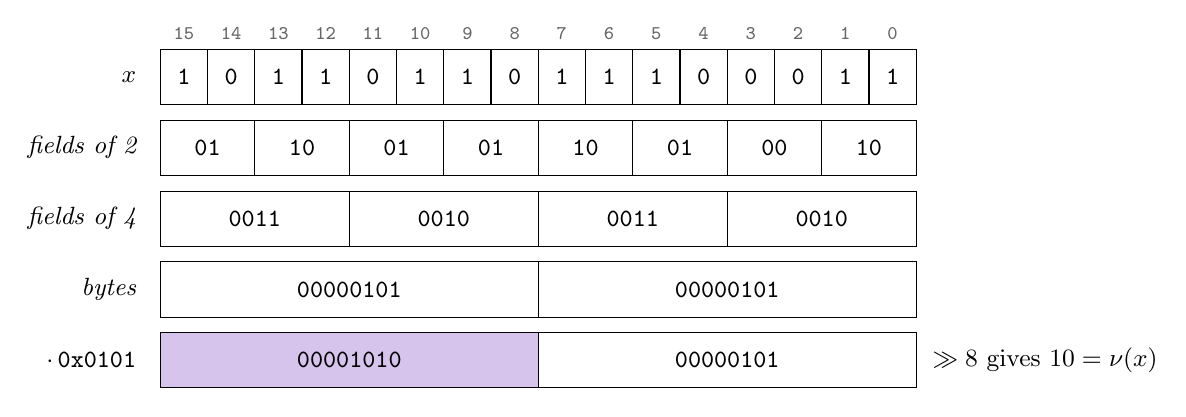
\begin{tikzpicture}[ads]
  % a row of k fields of width w, the first at (0,y), with their texts
  \newcommand{\fields}[4]{%
    \foreach \v [count=\i from 0] in {#4}
      \node[cell,minimum width=#2] at ($(\i*#2+0.5*#2,#1)$) {\v};
    \node[var,anchor=east] at (-3mm,#1) {#3};}
  \fields{0}{6mm}{$x$}{1,0,1,1,0,1,1,0,1,1,1,0,0,0,1,1}
  \fields{-9mm}{12mm}{fields of 2}{01,10,01,01,10,01,00,10}
  \fields{-18mm}{24mm}{fields of 4}{0011,0010,0011,0010}
  \fields{-27mm}{48mm}{bytes}{00000101,00000101}
  \fields{-36mm}{48mm}{$\cdot\,\mathtt{0x0101}$}{00001010,00000101}
  \node[touched,minimum width=48mm] at (24mm,-36mm) {00001010};
  \foreach \i in {0,...,15}
    \node[index] at ($(93mm-\i*6mm,5.5mm)$) {\i};
  \node[var,anchor=west] at (98mm,-36mm) {\textup{$\gg 8$ gives $10 = \nu( x )$}};
\end{tikzpicture}
\end{document}
